\documentclass[tikz]{standalone}

\usetikzlibrary{calc}

\begin{document}
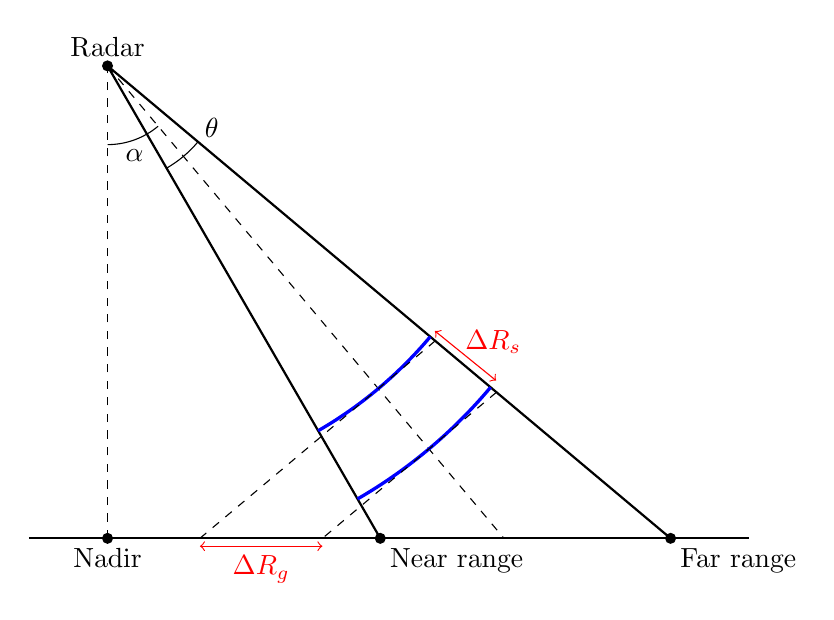
\begin{tikzpicture}

% Geometry
\def\radarHeight{6.0}
\def\lookAngle{40}       % measured from downward nadir
\def\beamWidth{20}

\pgfmathsetmacro{\lookAbsAngle}{-90+\lookAngle}

% Beam-edge angles relative to nadir
\pgfmathsetmacro{\nearAngle}{\lookAngle-\beamWidth/2}
\pgfmathsetmacro{\farAngle}{\lookAngle+\beamWidth/2}

% Ground intersections
\pgfmathsetmacro{\nearRange}{\radarHeight*tan(\nearAngle)}
\pgfmathsetmacro{\farRange}{\radarHeight*tan(\farAngle)}
\pgfmathsetmacro{\lookRange}{\radarHeight*tan(\lookAngle)}
\pgfmathsetmacro{\lookRadius}{\radarHeight/cos(\lookAngle)}

% Absolute TikZ angles
\pgfmathsetmacro{\edgeNear}{-90+\nearAngle}
\pgfmathsetmacro{\edgeFar}{-90+\farAngle}

% Pulse parameters
\def\RangeRes{1.0}
\pgfmathsetmacro{\pulseOne}{(\radarHeight-0.5)/cos(\lookAngle - \beamWidth/2)}            
\pgfmathsetmacro{\pulseTwo}{\pulseOne-\RangeRes}

\pgfmathsetmacro{\tanFarOne}{\pulseOne / cos(\beamWidth/2)}
\pgfmathsetmacro{\tanFarTwo}{\pulseTwo / cos(\beamWidth/2)}

\pgfmathsetmacro{\groundPulseOne}{(\pulseOne - \radarHeight*cos(\lookAngle))/sin(\lookAngle)}
\pgfmathsetmacro{\groundPulseTwo}{(\pulseTwo - \radarHeight*cos(\lookAngle))/sin(\lookAngle)}

% Coordinates
\coordinate (R) at (0,\radarHeight);
\coordinate (O) at (0,0);
\coordinate (N) at (\nearRange,0);
\coordinate (F) at (\farRange,0);
\coordinate (L) at (\lookRange,0);
\coordinate (G1) at (\groundPulseOne,0);
\coordinate (G2) at (\groundPulseTwo,0);
\coordinate (I1) at ($(R) + ({\edgeFar}:\tanFarOne)$);
\coordinate (I2) at ($(R) + ({\edgeFar}:\tanFarTwo)$);

% Ground
\draw[thick] (-1,0) -- (\farRange+1,0);

% Radar and nadir
\fill (R) circle (2pt) node[above] {Radar};
\draw[dashed] (O) -- (R);
\fill (O) circle (2pt) node[below] {Nadir};

% Beam boundaries
\draw[thick] (R) -- (N);
\draw[thick] (R) -- (F);

% Look direction
\draw[dashed]
    (R) -- (L);

% Near and far range points
\fill (N) circle (2pt) node[below right] {Near range};
\fill (F) circle (2pt) node[below right] {Far range};

% Look angle
\draw (R) ++(0,-1.0)
    arc[
        start angle=-90,
        end angle=\lookAbsAngle,
        radius=1.0
    ] node[midway, below] {$\alpha$};

% Beam width
\draw (R) ++({\edgeNear}:1.5)
    arc[
        start angle=\edgeNear,
        end angle=\edgeFar,
        radius=1.5
    ] node[xshift=5pt, yshift=5pt] {$\theta$};

% First pulse arc
\draw[
    very thick,
    blue
]
    (R) ++({\edgeNear}:\pulseOne)
    arc[
        start angle=\edgeNear,
        end angle=\edgeFar,
        radius=\pulseOne
    ];

% Second pulse arc
\draw[
    very thick,
    blue
]
    (R) ++({\edgeNear}:\pulseTwo)
    arc[
        start angle=\edgeNear,
        end angle=\edgeFar,
        radius=\pulseTwo
    ];

% Label for range resolution between pulse fronts
\draw[
    <->,
    red
]
    ($(R)+({\lookAbsAngle+\beamWidth/2 + 1}:\pulseOne)$) --
    node[xshift=10pt, yshift=5pt] {$\Delta R_s$}
    ($(R)+({\lookAbsAngle+\beamWidth/2 + 1}:\pulseTwo)$);

\draw[dashed] (I1) -- (G1);
\draw[dashed] (I2) -- (G2);

\draw[
    <->,
    red
]
    (\groundPulseOne, -0.1) --
    node[below] {$\Delta R_g$}
    (\groundPulseTwo, -0.1);

\end{tikzpicture}
\end{document}
